\section{A possible approach for a social network analysis}
\label{sec:network_analysis}

The possible methods to analyse a social network are diverse. The selection presented in this chapter is based on a choice of topics from the book \textit{Exploring Animal Social Networks}\cite{croft:07}. However, this chapter offers an introduction to these topics, since the complete analysis would deserve its own thesis. Furthermore, the genetic data to determine the kinship in the mice population, which obviously play a major role in the formation of social relationships and structures, is not available yet.  

As outlined in section \ref{subsubsec:export_options}, the available export formats of the network data using the \textit{miceminer} application, allow to use several different software packages to carry out network analyses. I decided to use the \textit{statnet}\cite{statnet:03} and \textit{igraph}\cite{igraph:06} packages for \lstinline|R|\cite{r:05}, mostly because I could program \lstinline|R| scripts an functions to simplify repetitive processes.


The sex is the only attribute data for the mice available in the exported network data so far. Therefore the following approach will focus on the differences betwwen the inner- and inter-gender relationships.

\subsection{Data selection \& edge filtering}
\label{subsec:data_selection}

The data has been retrieved with a minimal time two mice must have spent together (see \ref{subsec:graph_concept} and \ref{subsec:graph_config}) of 3 hours (6 minutes/day) and 20 hours (1 hour/day) and range from June 2008 to June 2009.Since the data is exported per month, we obtain data for 26 networks (13 for each limit).

The selection of the two thresholds is based on general considerations. Namely, to have whatever kind of social relation, two mice must spend at least 5 minutes per day ($\frac{5\:min}{day} * 30\:days\:=\:150\:min\:=\:2.5\:hours \approx 3\:hours$) together. To build a biologically more justifiable relationship, however, the mice should spend at least 1 hour per day ($\frac{1\:hour}{day} * 30\:days\:=\:30\:hours$) together. The process of determining the right threshold is called \textit{edge filtering}. 

Figure \ref{fig:meeting_frequency_januray} shows a histogram of the monthly meeting duration for the network data of January 2009. Remember that the edge values are calculated as the sum of the time the two mice spent together during the month (\ref{subsec:graph_concept}).

\begin{figure}[htpb]
\begin{center}
  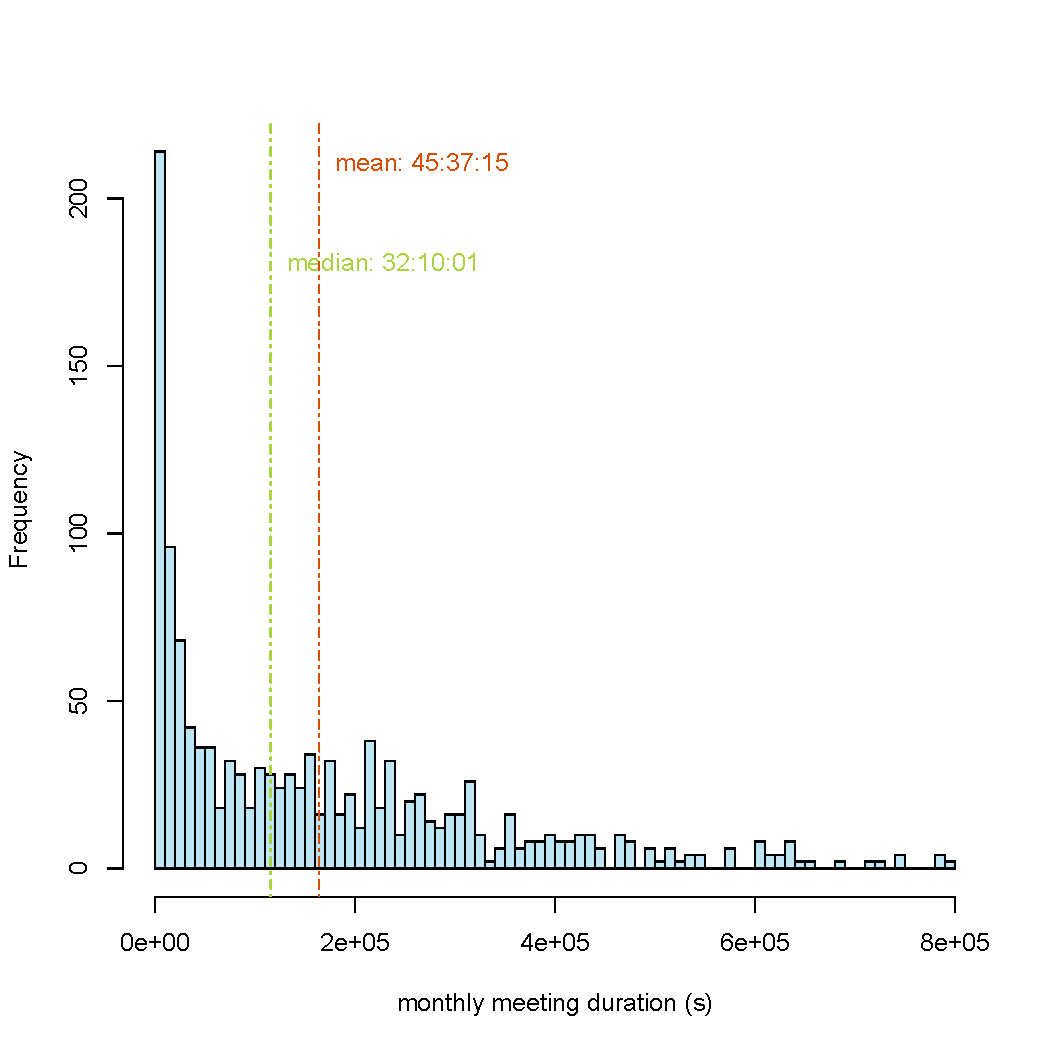
\includegraphics[width=.75\textwidth]{assets/pdf/meeting_frequency_january.pdf}
  \caption[Histogram of monthly meeting duration]{Meeting duration distribution for the network data for January 2009. Additionaly, the median and mean values (hh:mm:ss) are indicated.}
  \label{fig:meeting_frequency_januray}
\end{center}
\end{figure}   

\subsection{Visual exploration}
\label{subsec:visual_exploration}

The network visualizations in this section have been created using the \textit{network}\cite{network:08} package, which is part of the \textit{statnet}\cite{statnet:03} library. The layout is determined by the \textit{Fruchterman \& Reingold}\cite{fruchterman:91} algorithm, which is a force directed layouter similar to the one used in the \textit{miceminer} implementation (see \ref{subsec:graph_explore}).

Other than the visulization in the \textit{miceminer} application, the \textit{network} package allows to visualize all the network components at the same time and is flexible in terms of the selection of the data to display or the highlighting of specific elements in the visualization.    

Pictured in figures \ref{fig:graph_january_3h} and  \ref{fig:graph_january_30h} are the networks for January 2009 with the edge filter threshold set to 3 hours and 30 hours respectively. Although the edges within the components of the network are not visible, the amount of \textit{isolates}, nodes with a degree of zero, is noticeable higher in the network with an edge filter value set to 30 hours.

\begin{figure}[htpb]% 
	\centering 
	\subfloat[Network with edge filter set to 3h][Edge filter treshold set to 3 hours.]{
					\label{fig:graph_january_3h} %
					
					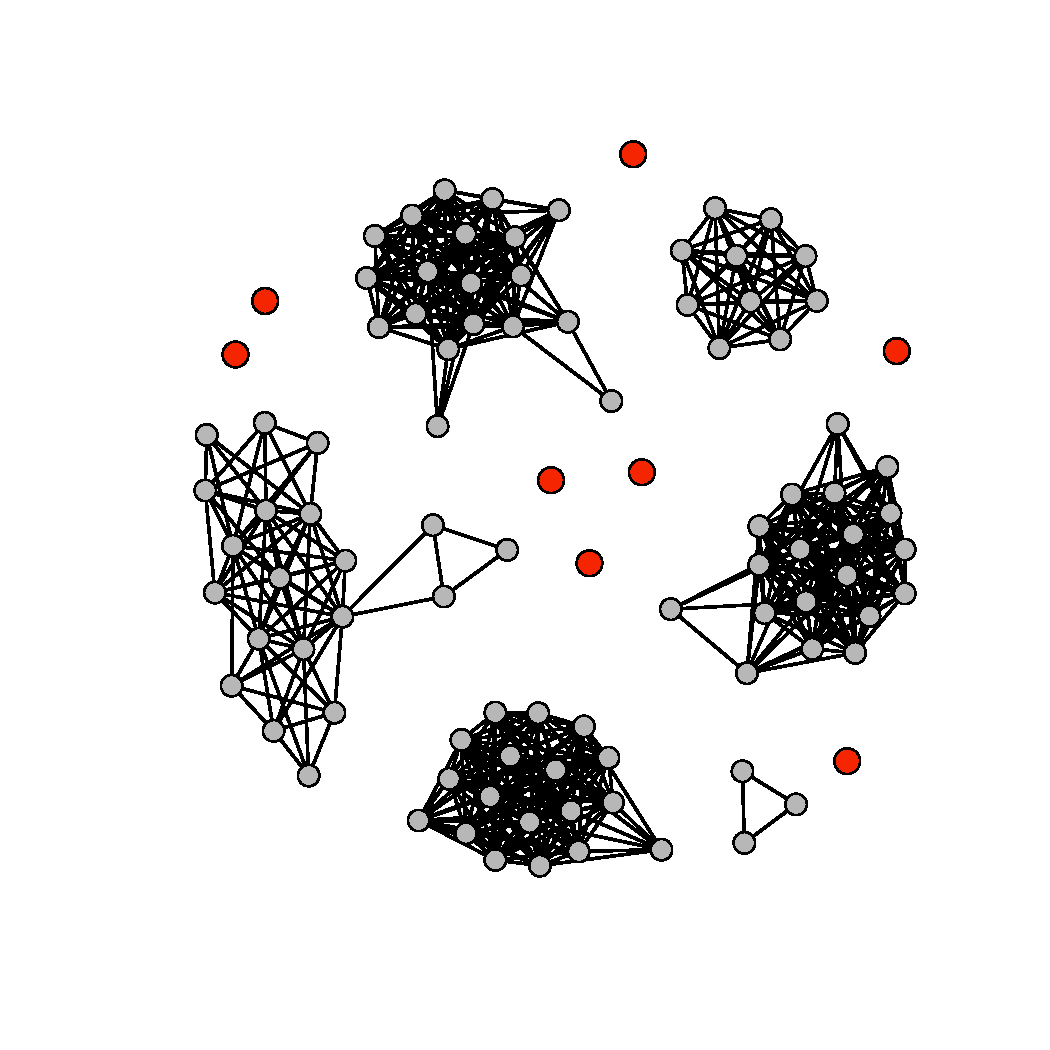
\includegraphics[width=.45\textwidth]{assets/pdf/graph_january_3h.pdf}
				}% 
	\qquad 
	\subfloat[Network with edge filter set to 30h][Edge filter threshold set to 30 hours.]{
					\label{fig:graph_january_30h}%
					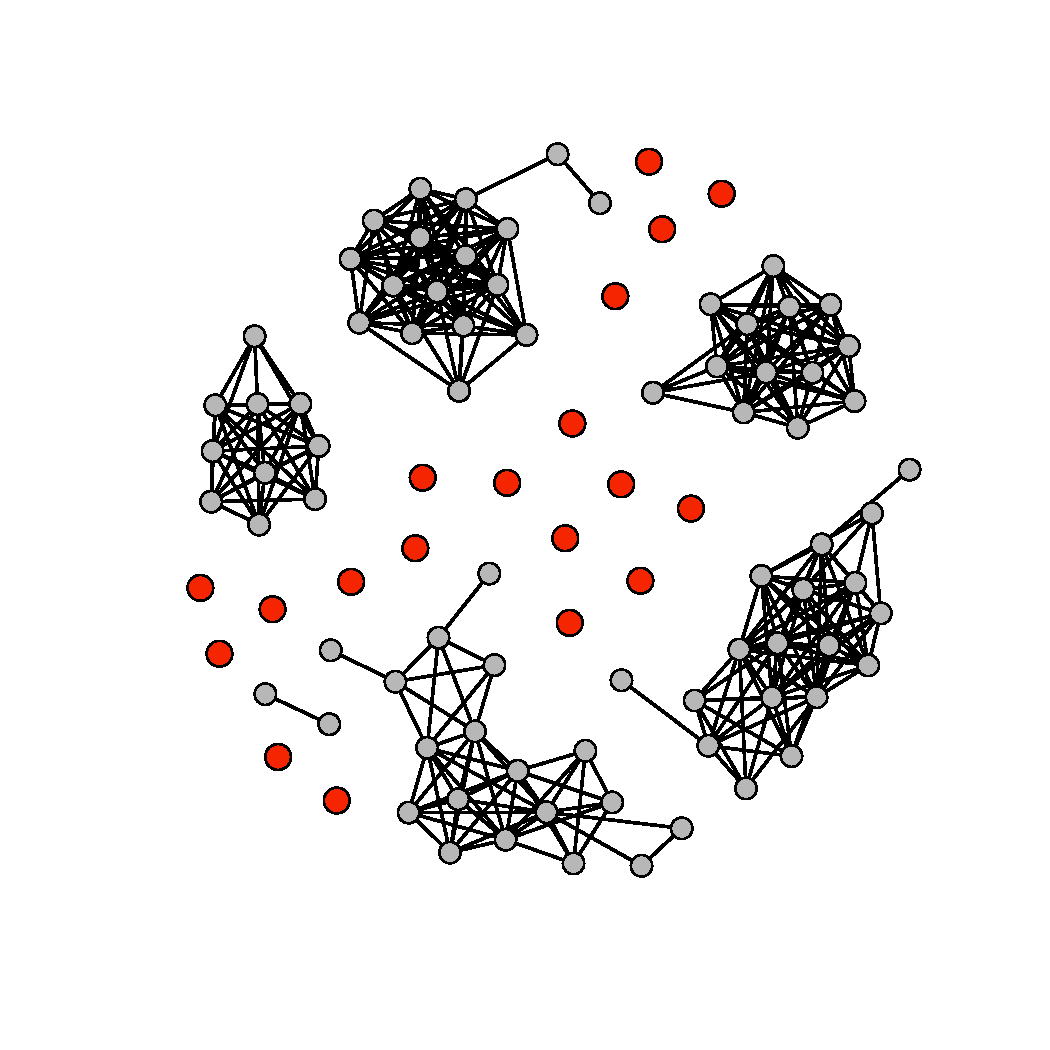
\includegraphics[width=.45\textwidth]{assets/pdf/graph_january_30h.pdf}
				} 
	\caption[Network visualizations with different edge filter values]{A visualization of the network for Januray 2009 with the edge filter treshold set to 3 hours \subref{fig:graph_january_3h} and 30 hours \subref{fig:graph_january_30h}. Isolates are highlighted red.} 
	 
\end{figure}    

To draw some clearer image of the network and since we are interested in the differences of the inner- and inter-gender networks, the nodes in figures \ref{fig:graph_january_3h_gender} and \ref{fig:graph_january_30h_gender} are colored based on their gender.

\begin{figure}[htpb]% 
	\centering 
	\subfloat[Network with edge filter set to 3h and node coloring based o the gender][Edge filter treshold set to 3 hours.]{
					\label{fig:graph_january_3h_gender} %
					
					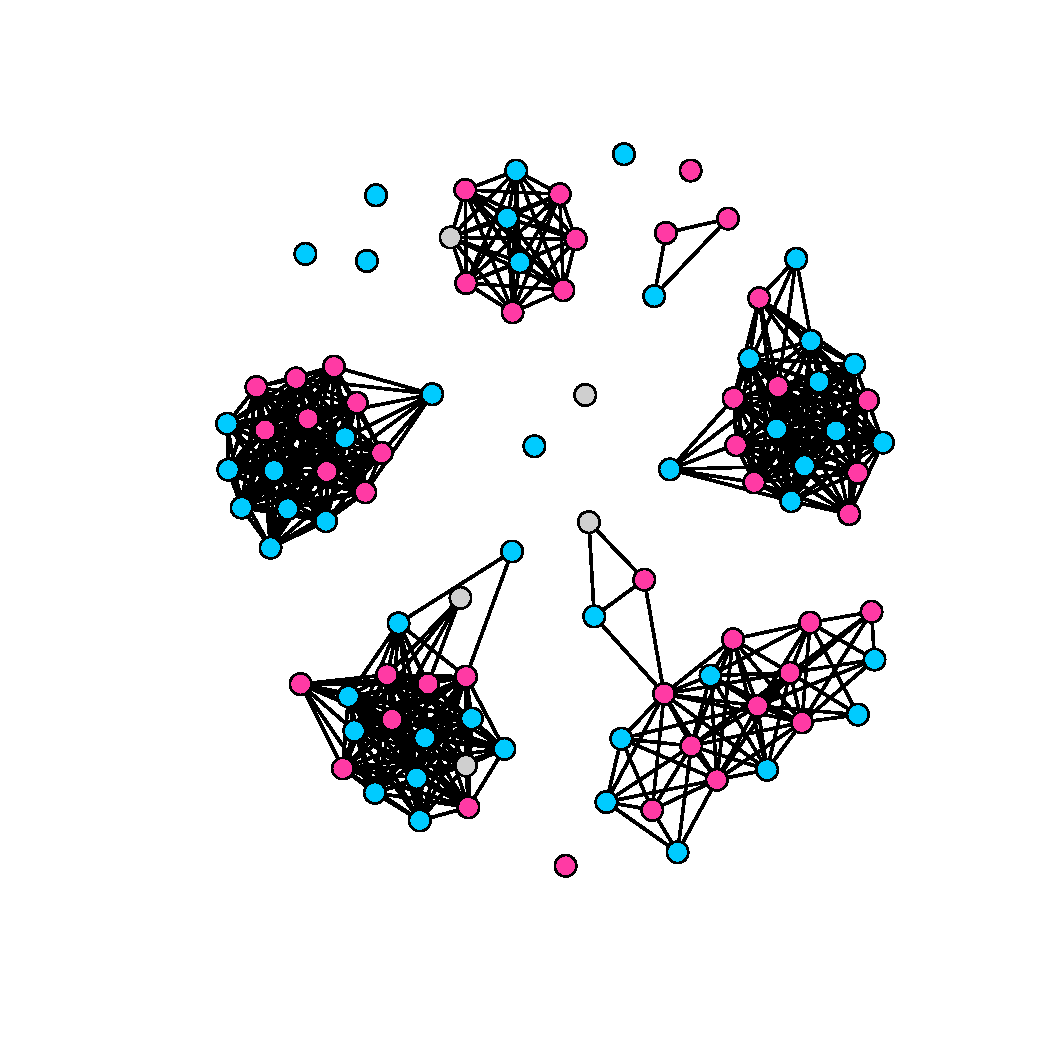
\includegraphics[width=.45\textwidth]{assets/pdf/graph_january_3h_gender.pdf}
				}% 
	\qquad 
	\subfloat[Network with edge filter set to 3h and node coloring based o the gender][Edge filter threshold set to 30 hours.]{
					\label{fig:graph_january_30h_gender}%
					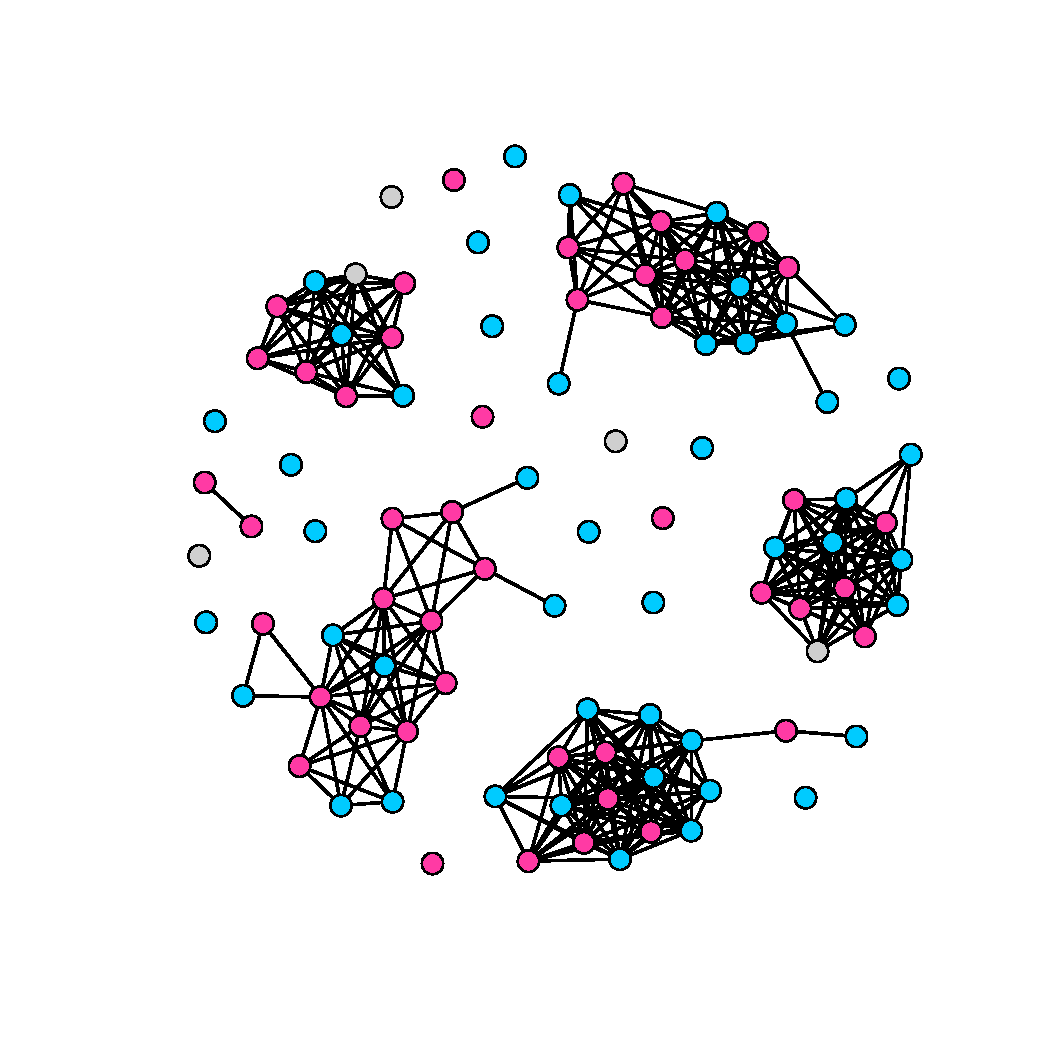
\includegraphics[width=.45\textwidth]{assets/pdf/graph_january_30h_gender.pdf}
				} 
			
	\caption[Network visualizations with different edge filter values]{A visualization of the network for Januray 2009 with the edge filter treshold set to 3 hours \subref{fig:graph_january_3h} and 30 hours \subref{fig:graph_january_30h}. Additionally, the nodes are colored based on the gender. Female mice are colord pink, males light blue, and mice with an unknown gender grey.} 
	 
\end{figure}

Still, the entanglement of the edges within the network components do not allow for a conclusion about specific edges. However, figure \ref{fig:graph_january_30h_gender} exposes a tendency that female mice are located more in the center of the components, whereas male mice are found in the preiphery. Furthermore, the same figure reveals, that the quantity of the male \textit{isolates} is higher then the one for female mice. This supports the assumption, that females are stronger networked as the males, and can be elaborated by visualizing the inner-gender (figures \ref{fig:graph_january_3h_ff} and \ref{fig:graph_january_30h_mm} ) and inter-gender (figure \ref{fig:graph_january_30h_fm}) networks. The visual comparison clearly unveils the higher connectivity within the female mice.

\begin{figure}[htpb]% 
	\centering 
	\subfloat[Network of female mice][Network of female mice]{
					\label{fig:graph_january_3h_ff} %
					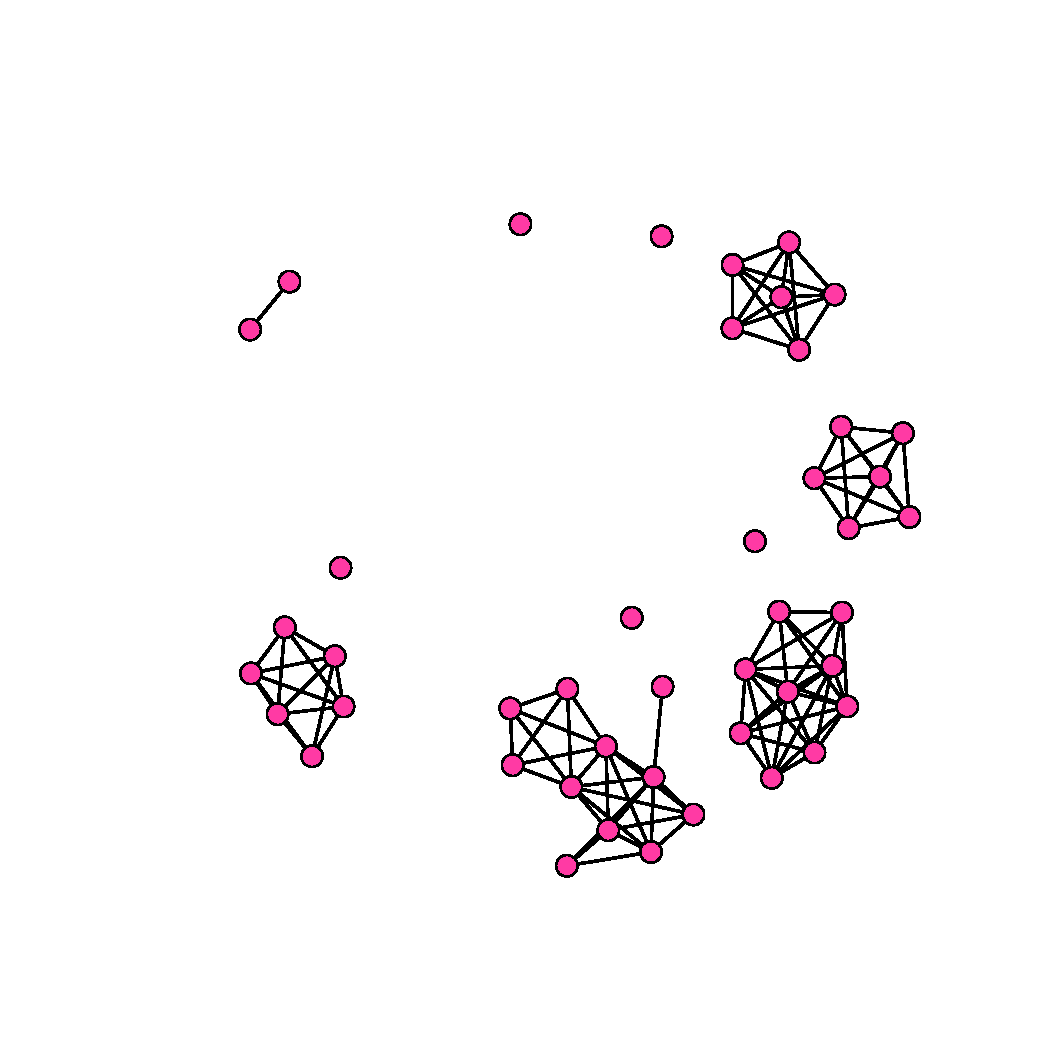
\includegraphics[width=.45\textwidth]{assets/pdf/graph_january_30h_ff.pdf}
				}
	\qquad 
	\subfloat[Network of male mice][Network of male mice]{
					\label{fig:graph_january_30h_mm}%
					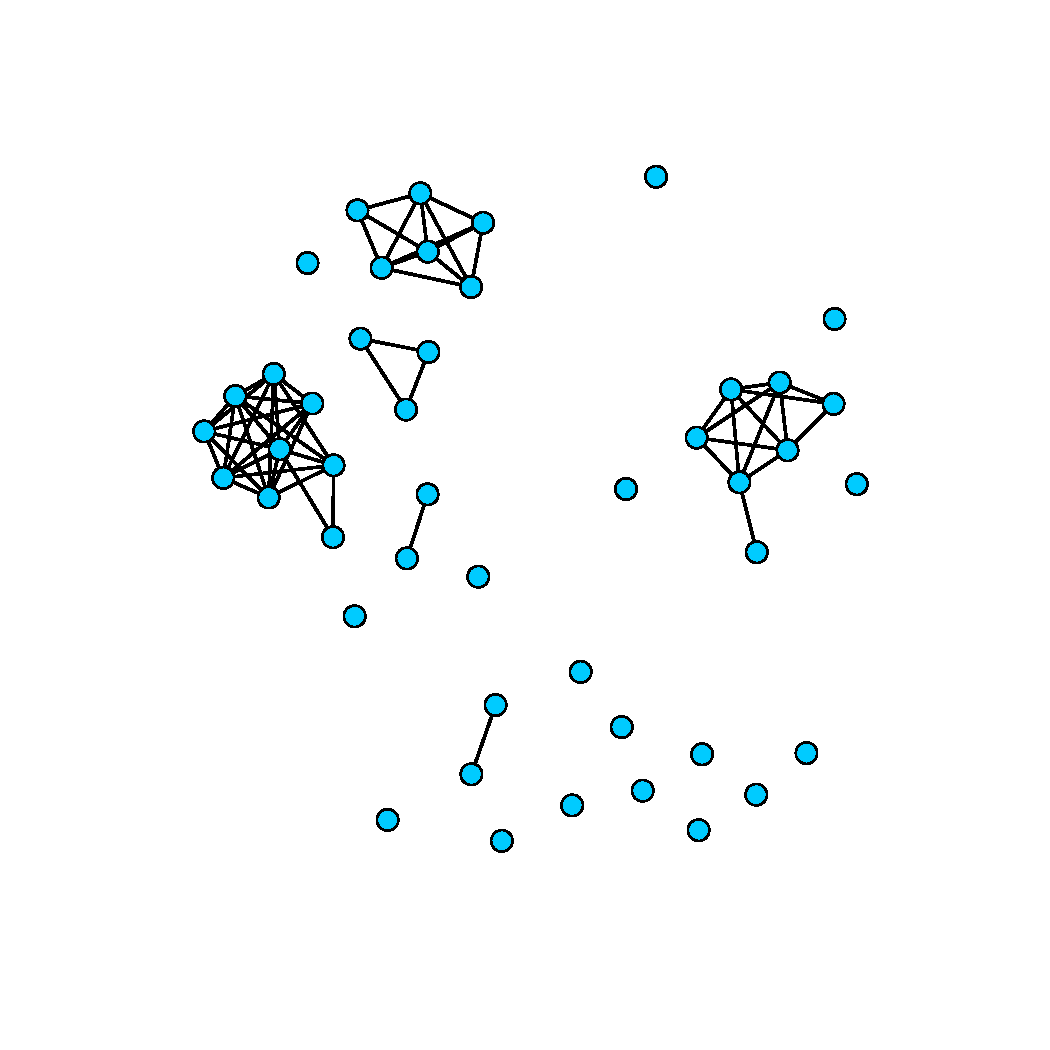
\includegraphics[width=.45\textwidth]{assets/pdf/graph_january_30h_mm.pdf}
				}
	\qquad  
	\subfloat[Inter-gender network][Inter-gender network]{
					\label{fig:graph_january_30h_fm}%
					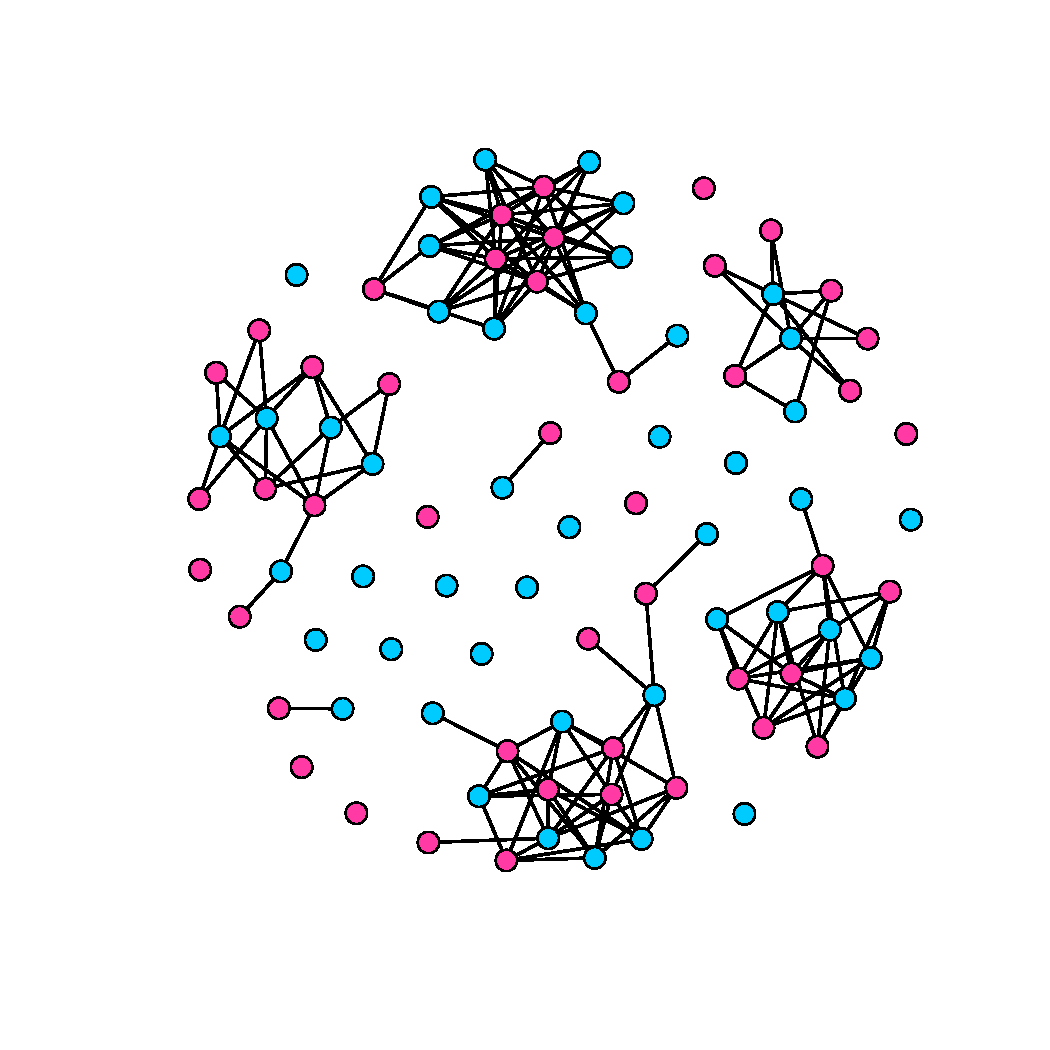
\includegraphics[width=.45\textwidth]{assets/pdf/graph_january_30h_fm.pdf}
				} 
				
	\caption[Network visualizations of the inner- and inter-gender networks]{Visualizations of the inter- and inner-gender networks for January 2009 with the edge filter value set to 30 hours.} 
	 
\end{figure}

After visually examining the general network structure, let's adapt the visualization to emphasize the role of the individuals depending on the node based measures introduced in section \ref{subsubsec:node_based} (see figures \ref{fig:graph_january_30h_apl} - \ref{fig:graph_january_30h_betweenness}). 

\begin{figure}[htpb]% 
	\centering 
				
	\subfloat[Network visualization where the node size is proportional to the average path length of the node][Network visualization where the node size is proportional to the average path length of the node (larger node size means lower value).]{
					\label{fig:graph_january_30h_apl}%
					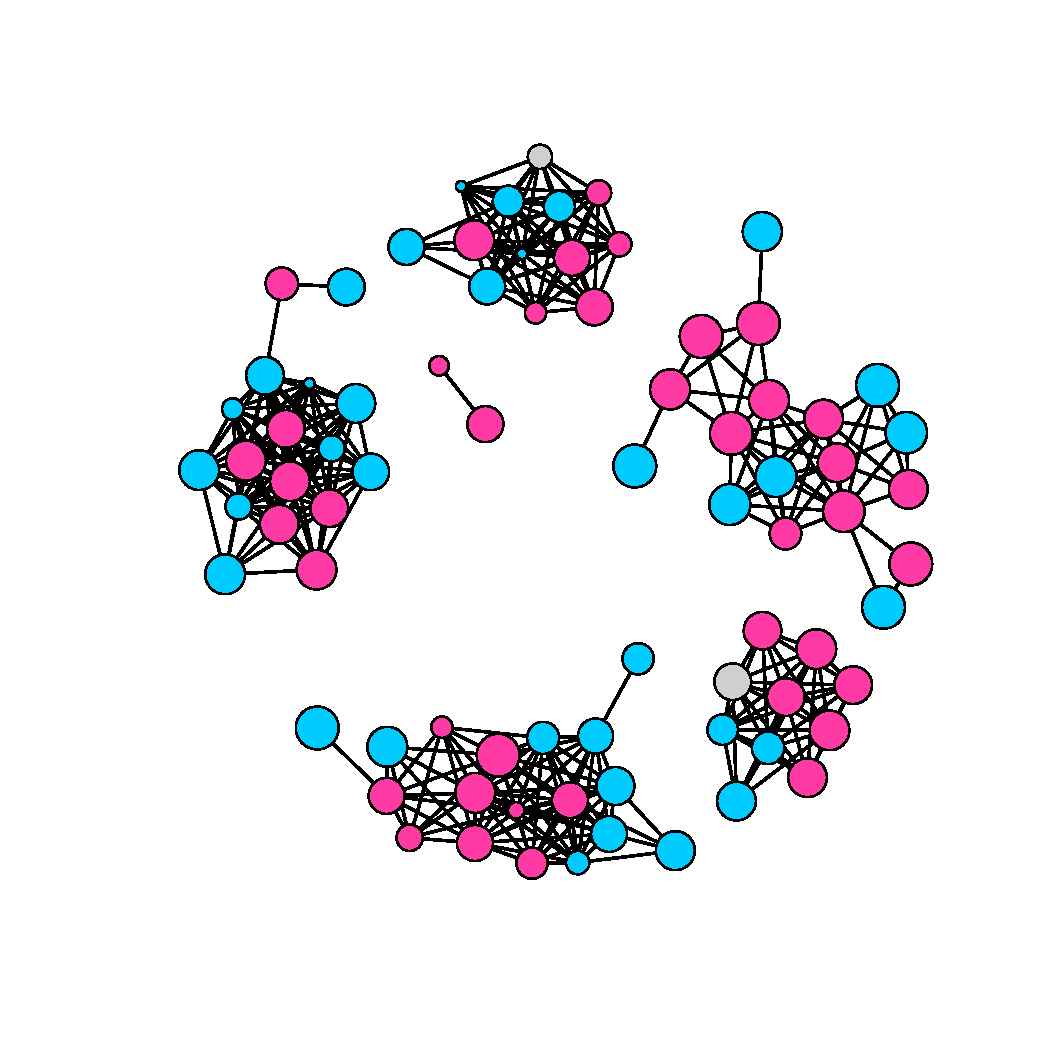
\includegraphics[width=.45\textwidth]{assets/pdf/graph_january_30h_apl.pdf}
				}
	\qquad 
	\subfloat[Network visualization where the node size is proportional to the clustering coefficient of the node][Network visualization where the node size is proportional to the clustering coefficient of the node.]{
					\label{fig:graph_january_30h_cc}%
					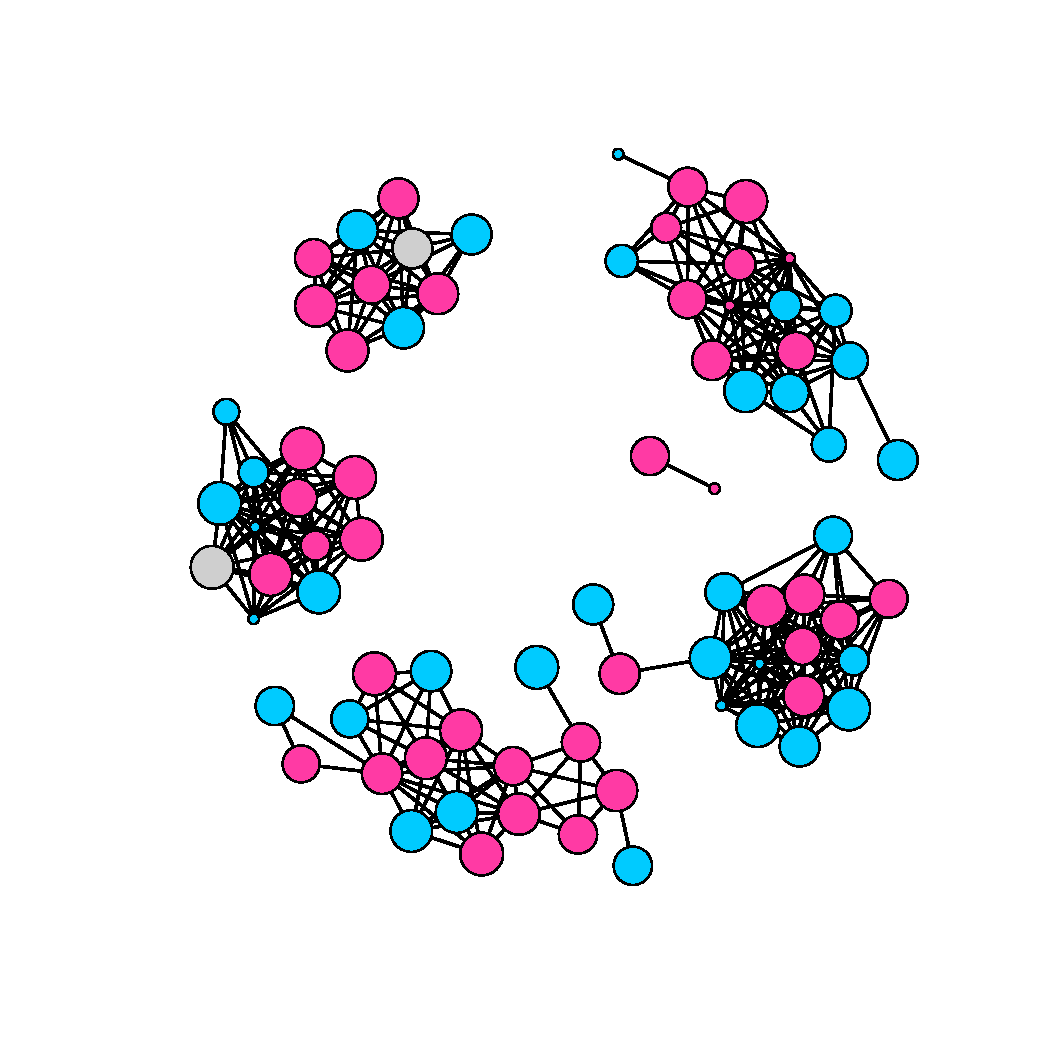
\includegraphics[width=.45\textwidth]{assets/pdf/graph_january_30h_cc.pdf}
				}
	\qquad 			
	\subfloat[Network visualization where the node size is proportional to the degree of the node][Network visualization where the node size is proportional to the degree of the node.]{
					\label{fig:graph_january_3h_degree}
					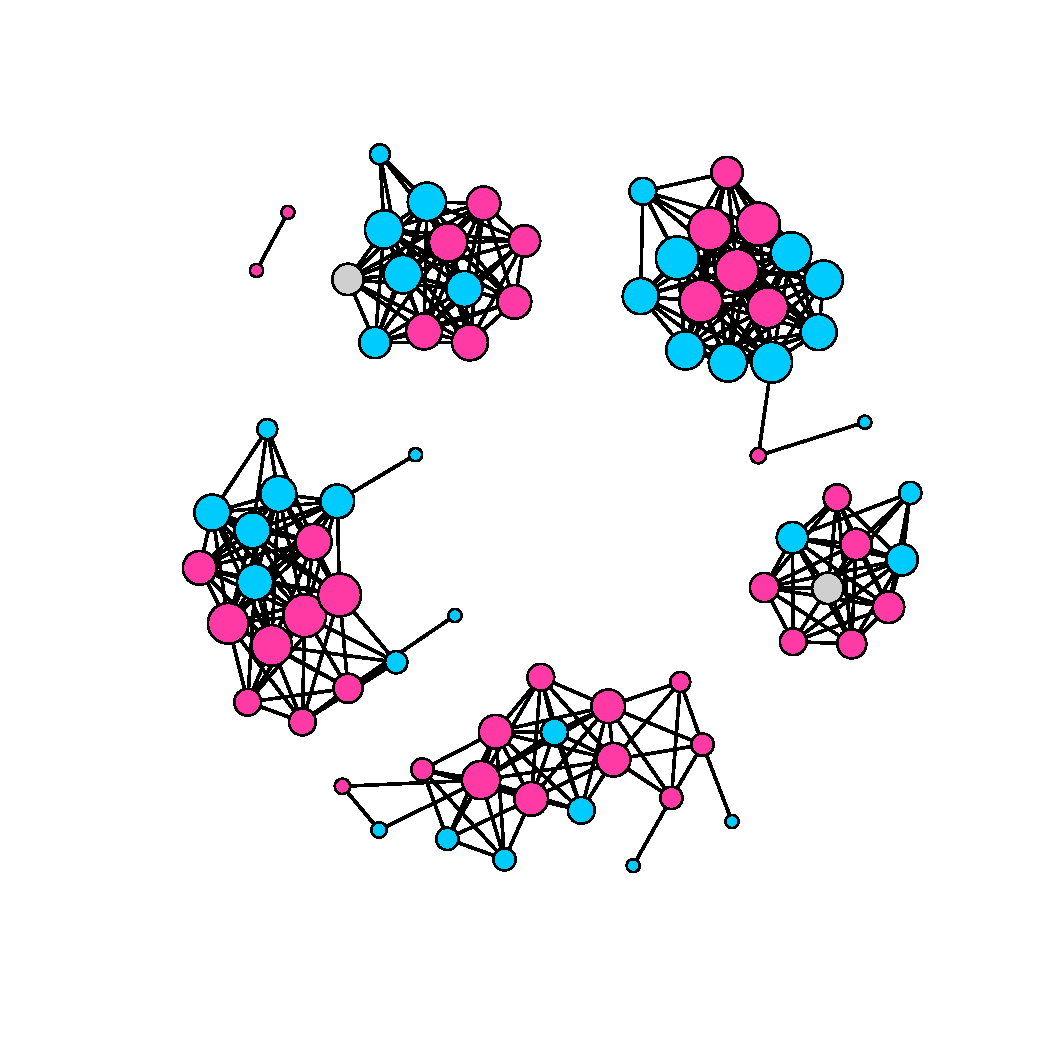
\includegraphics[width=.45\textwidth]{assets/pdf/graph_january_30h_degree.pdf}
				}
	\qquad 
	\subfloat[Network visualization where the node size is proportional to the betweenness of the node][Network visualization where the node size is proportional to the betweenness of the node.]{
					\label{fig:graph_january_30h_betweenness}
					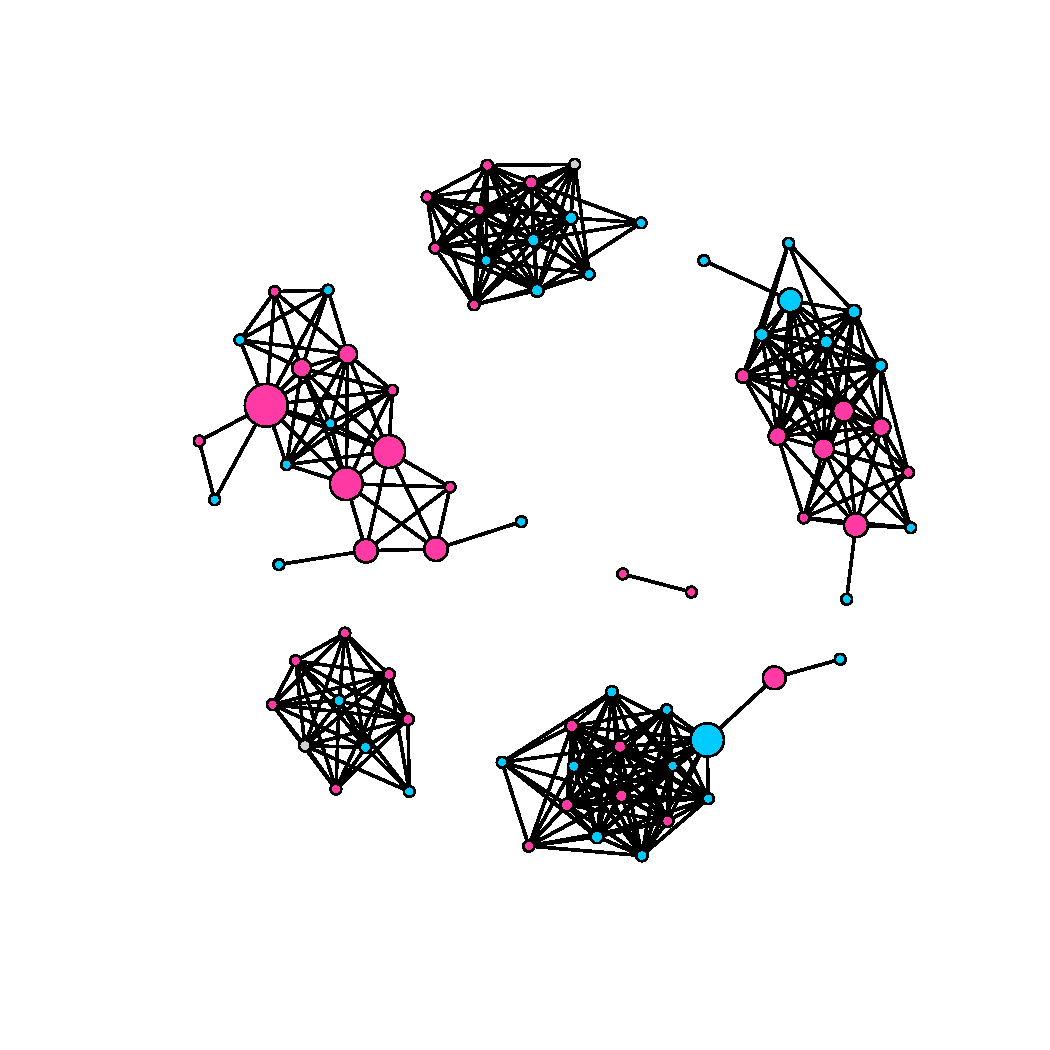
\includegraphics[width=.45\textwidth]{assets/pdf/graph_january_30h_betweenness.pdf}
				} 		 				
		
	\caption[Network visualizations where the node size is proportional to node based measures]{Network visualizations for January 2009, where the node size is proportional to a node based measure.} 
	 
\end{figure}

Except for the visualization based on the betweenness values (figure \ref{fig:graph_january_30h_betweenness}), no nodes stand out. This is coherent to the observation, that the network components are strongly connected. Consequently, the clustering coefficient is high, and the average path lengths are low due to the existance of the many edges.  

A closer look at figure \ref{fig:graph_january_30h_betweenness}, however, reveals, that most of the nodes with a high betweenness value are \textit{Cut-Points} as well. A \textit{Cut-Point} is a node whose deletion increase the number number of components in the network\cite{pajek:03}. In and of itself, these nodes are very interesting, since they act as a bottleneck when information has to be passed from one group to the other. In this case however, all the \textit{Cut-Points} connect at most two other nodes to the network (see figure \ref{fig:graph_january_3h_cutpoints}). Hence, we focus on the nodes with a high betweeness value\footnote{8 Nodes with a betweenness value bigger than 15 have been included in the list.}, which are not \textit{Cut-Points}\footnote{7 \textit{Cut-Points} have been found using the sna\cite{sna:09} package for \lstinline|R|.} (see figure \ref{fig:graph_january_3h_cutpoints_betweenness}). The resulting visualization discovers two female mice. This idea to identify potentially interesting indviduals will be picked up in section \ref{subsec:longitudinal_analysis}. 

\begin{figure}[htpb]% 
	\centering 
	\subfloat[Network visualization with highlighted \textit{Cut-Points}][Network visualizations for January 2009 with highlighted \textit{Cut-Points}.] {
		\label{fig:graph_january_3h_cutpoints}
  		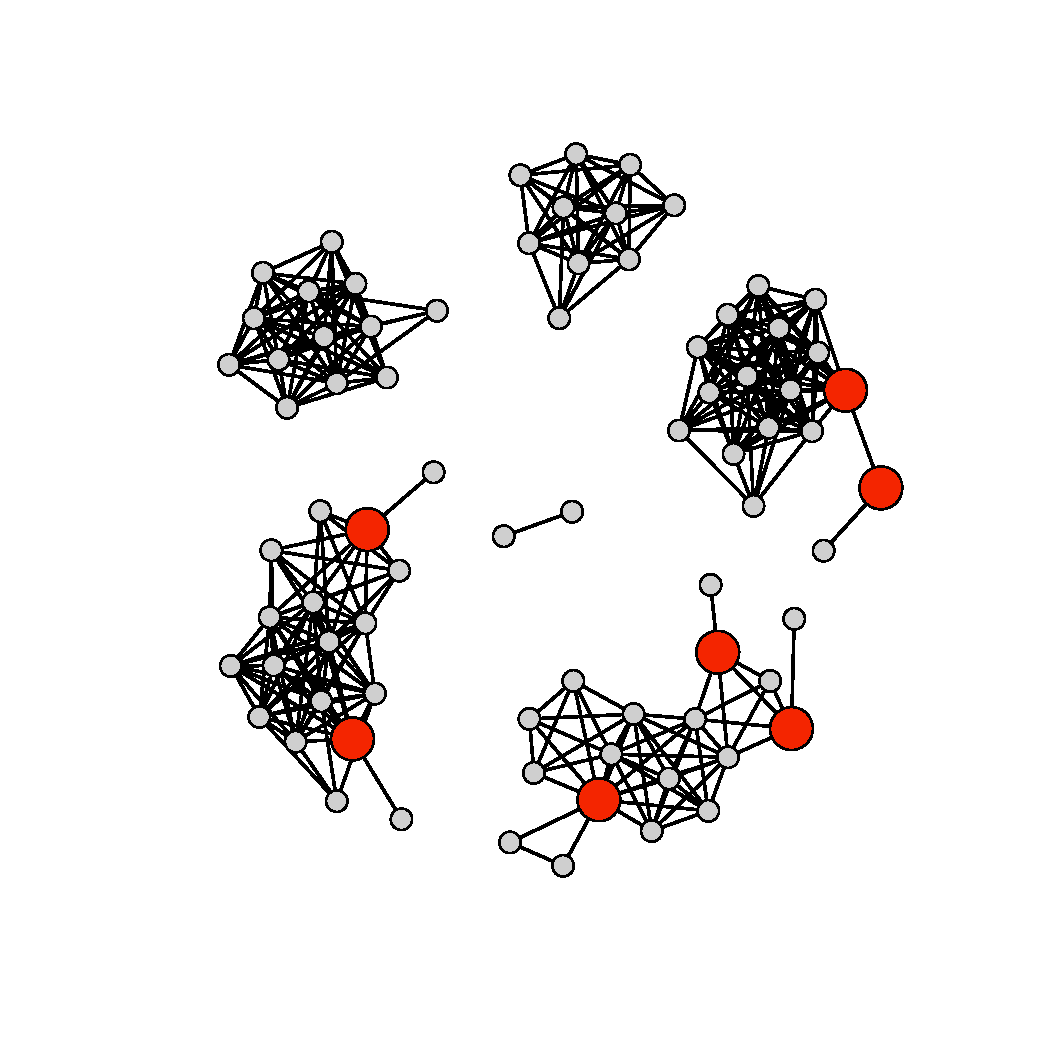
\includegraphics[width=.45\textwidth]{assets/pdf/graph_january_30h_cutpoints.pdf}
	}
	\qquad
	\subfloat[Network visualization with nodes highlighted, that have a high betweenness value and are not \textit{Cut-Points}][The larger nodes have a high betweenness value but are not \textit{Cut-Points}.] {
 		\label{fig:graph_january_3h_cutpoints_betweenness}
 		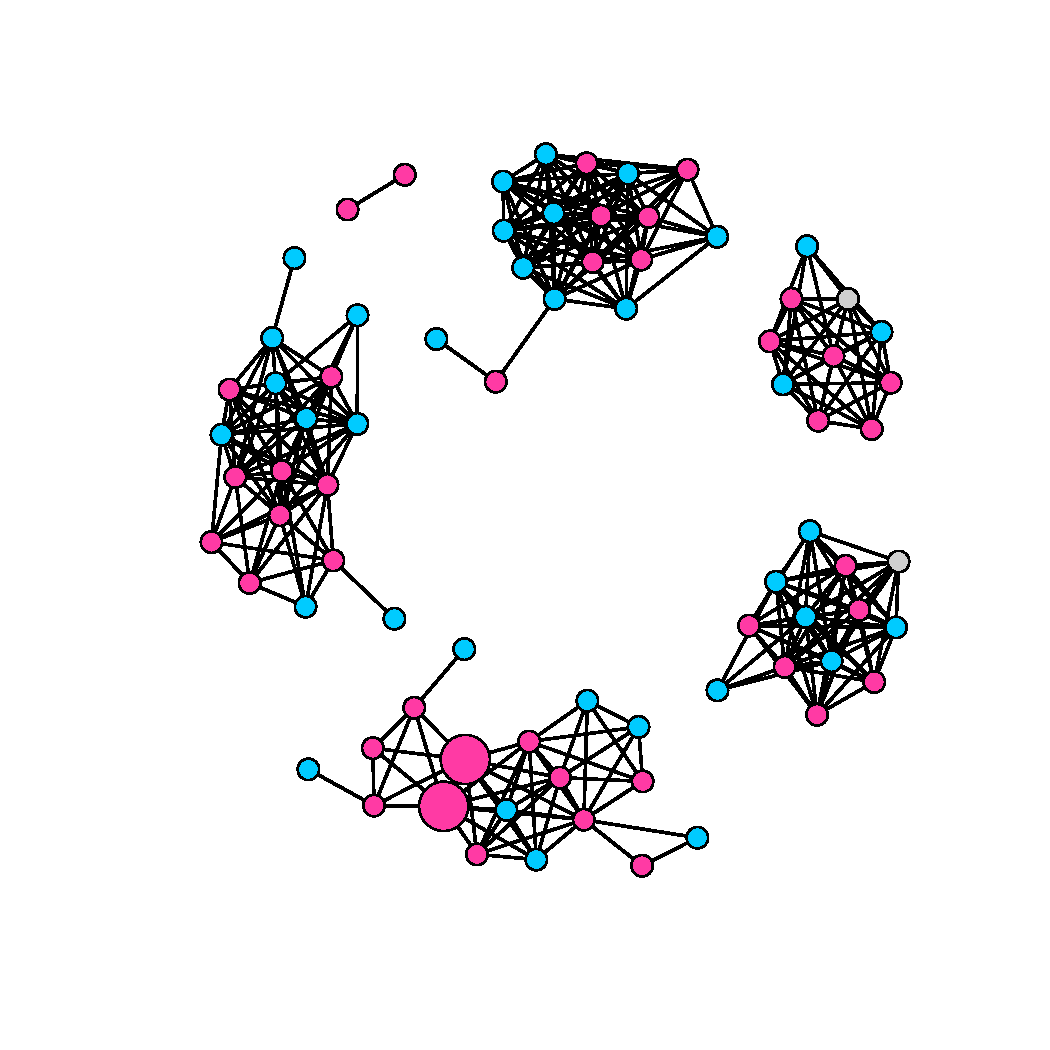
\includegraphics[width=.45\textwidth]{assets/pdf/graph_january_30h_cp_bet.pdf}
  	}
  	
  	\caption[Network visualization of \textit{Cut-Points} and such with a high betweeness value which are not \textit{Cut-Points}]{Identifying \textit{Cut-Points} \subref{fig:graph_january_3h_cutpoints} and such nodes with a high betweenness value which are not \textit{Cut-Points} \subref{fig:graph_january_3h_cutpoints_betweenness}.}
  	
\end{figure}


\subsection{Quantitative analysis}
\label{subsec:quantitative_analysis}



\subsection{Longitudinal analysis}
\label{subsec:longitudinal_analysis}




\subsection{Network modeling}
\label{subsec:network_modeling}

\subsubsection{Longitudinal exploration of the network data}
\label{subsec:longitudinal}
No statistics.

\begin{mylist}
\item Trace special mice or positions (brokers, cut-points) over a period of one year.
\item How the network changes over the time based on the node based measures.
\end{mylist} 

\subsection{Statistical modeling of a network}
\label{subsec:exploratory}

\begin{mylist}
\item ERGM: Introduction
\item ERGM: simple modelling approach
\item ERGM: outline the possibilities with more attribute data
\item ERGM: outline the possibilities with weighted edges
\end{mylist}

\subsubsection{Longitudinal exploration of the network data by use of ERGM and Hammond Distances}

Comparing the networks using the hammond distance.
